\documentclass{article}
\usepackage{geometry}
\usepackage{flafter}
\geometry{letterpaper, portrait, margin=1in}

\usepackage{hyperref}
\hypersetup{
    colorlinks=true,
    linkcolor=black,
    filecolor=magenta,
    urlcolor=blue,
}

\usepackage{graphicx}
\graphicspath{ {images/} }

\usepackage{tcolorbox}
\usepackage{textcomp}
\usepackage{gensymb}
\usepackage{indentfirst}

\newcommand{\ans}{$\rule{1.5cm}{0.15mm}$}

\title{RoboJackets Electrical Training Week 4 Lab Guide}
\author{Arthur Siqueira}
\date{\today\\v1.0}

\begin{document}
\maketitle{}
\setcounter{tocdepth}{2}
\tableofcontents
\pagebreak

%Everything below is for you to edit. Code above sets up the general formatting for the document

\section{Background}
This week, we are addressing how to create the Board Layout design of a PCB. There are many specific details to the art of designing a PCB, but our main intention is to introduce you to the basics of it all. Every time that you want to make a PCB for attending your specific application, you need to go through some steps and that's not different in RoboJackets. Every team has several different boards that support either their main robots or parallel projects that are relevant for the team. On this lab, we will design the PCB Layout of the Firmware Training Board. This is the same board which you all have made the schematic last week.

\section{Objective}
\subsection{Board dimensions}
The board size depends a lot on the application and on the constraints set by the components that will go on the board. For example, smaller boards are preferable if you want to put your board inside a tight system like a robot (and in most cases actually), however if the end-application don't have many physical constraints, you can make your board bigger and thus make it easier to routing traces on it and soldering the components after the PCB is manufactured.

\subsection{Optimize User Experience}
In the end, you want your board to look good and to be informative enough for the end-user.
\subsubsection{Silkscreen}
Use the Silkscreen layers to put information for people assembling or using your board. In general, people tend to put less information than it would be helpful, however, don't put too much unnecessary silkscreen to a point of polluting the board view.
\subsubsection{Space between components}
Specially if your board is going to be soldered, remember to put some space between components so that if it needs to be assembled or debugged, the user can easily take out or put components.
\pagebreak

\section{Relevant Information}
\subsection{Datasheet!}
You thought that you only would need to analyze datasheets while doing the schematics and choosing the components for your board? Nope! The datasheet has very useful information on how to do the layout. It will suggest the positioning of certain supportive discrete components (like resistors and capacitors) and how should the polygons and traces around the main component look like. In fact, it will commonly show you an example of a working Board Layout like in Figure 1.

\begin{figure}[ht]
	\center
	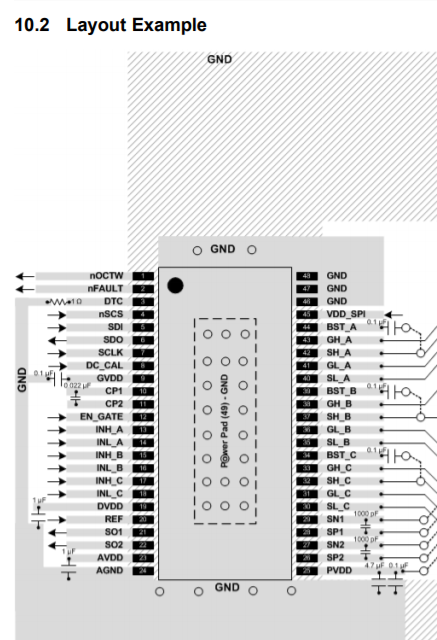
\includegraphics[width=0.6\textwidth, keepaspectratio]{images/layout.png}
	\caption{Layout example from a component's (DRV8303) datasheet. Note it suggests the positioning of capacitors and the width of certain traces.}
	\label{fig:layout}
\end{figure}

\subsection{Terminology}
Here are some terms you should be comfortable with:
\begin{itemize}
\item Layers: Different cattegories for elements in the board. Here are all the Eagle layers explained:

\href{https://www.autodesk.com/products/eagle/blog/every-layer-explained-autodesk-eagle/}{https://www.autodesk.com/products/eagle/blog/every-layer-explained-autodesk-eagle/}

\item Trace: The filament of copper that connects pins around your board.
\item Via: Copper platted hole that goes from top to bottom layers and passes by all the other layers. 
\item Polygon: Region of board designated to be entirely filled with copper and thus can be used to connect pins.
\end{itemize}

\section{Guided Lab}
\subsection{Open the file}
\subsubsection{Find Template Schematic}
On the electrical-training repository of RoboJackets, either download the .zip file of the entire repository and open the lab/Week4 folder; or git clone the repository and access the same folder. 
\subsubsection{Switch to Board Layout view}
Normally, the folder with the Eagle files would have both .sch (Schematics) and .brd (Board Layout) files, but I deleted the .brd file so you could first open the .sch file and switch to an empty .brd file. So do that! Open the .sch file and then press on the "SCH/BRD" button on the top, see Figure 2.

\begin{figure}[ht]
	\center
	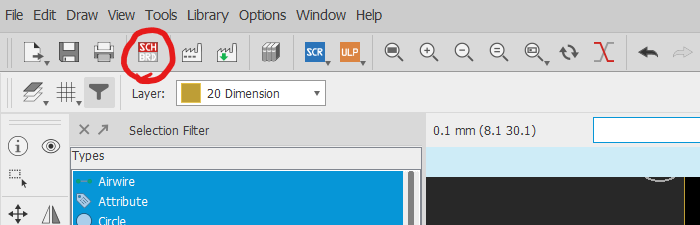
\includegraphics[width=0.7\textwidth, keepaspectratio]{images/SCH.png}
	\caption{This is the button you should press!}
	\label{fig:SCH}
\end{figure}
\subsection{Set the Design Rules}
You will need to set the constraints for the board layout you want to create. Those constraints are commonly set due to limitations of the PCB manufacturers. For instance, some manufacturers can drill 0.1 mm holes on your PCB, but some others are only able to do holes bigger than 0.3 mm.

So, for this lab, you should load the design rules of JLCPCB which you can find on the eagle-libraries repository that you should have downloaded/cloned on Week 2.

For doing that, you will need to click on the DRC Tool on the left toolbar and then click on "Load...". After that, you will be prompted to select a file from your computer, so select "JLCPCB (2 layer)" under "eagle-libraries/design rules/JLCPCB/JLCPCB (2 layer)". Done! You don't need to press "Check" just yet, leave that for the end.
\pagebreak
\subsection{Shape the board}
Since this board will be attached to the top of an Arduino Uno by connecting to all of its exposed pins, our main constraint is going to be those predefined pins. Then, we will preferably want to make the board smaller or the same size as the Arduino Uno board like the example on Figure 4. For that, you can also use the Miter tool to shape the corners.

\begin{figure}[ht]
	\center
	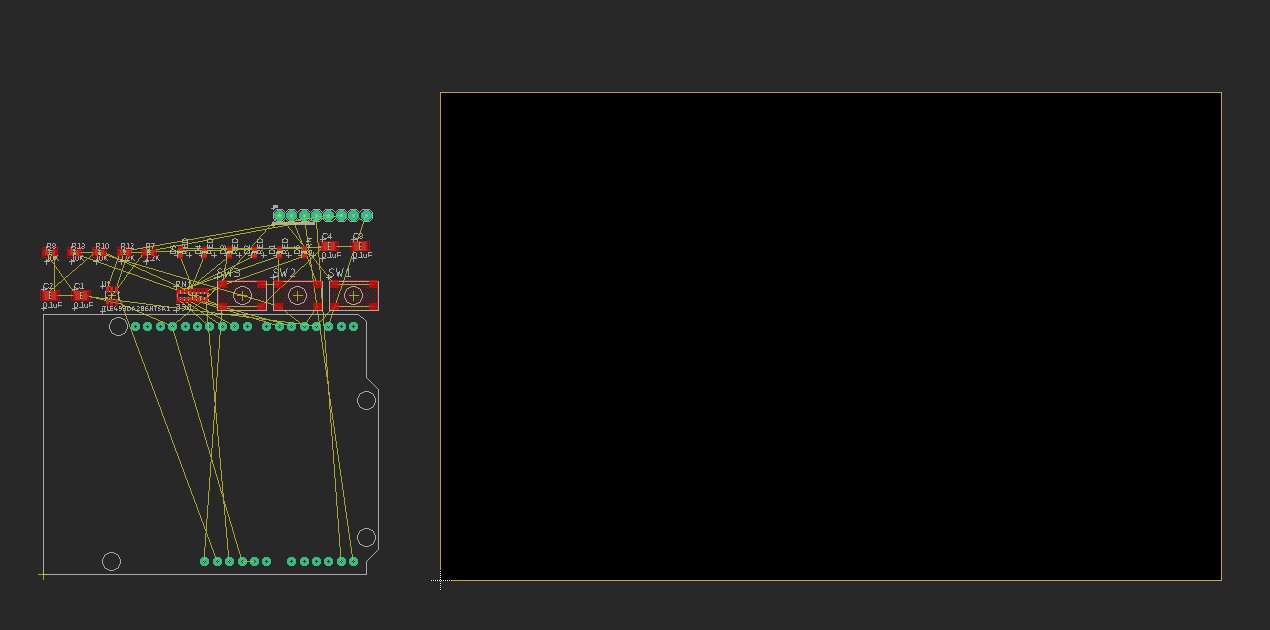
\includegraphics[width=0.7\textwidth, keepaspectratio]{images/start.png}
	\caption{You will start with this view.}
	\label{fig:start}
\end{figure}

\begin{figure}[ht]
	\center
	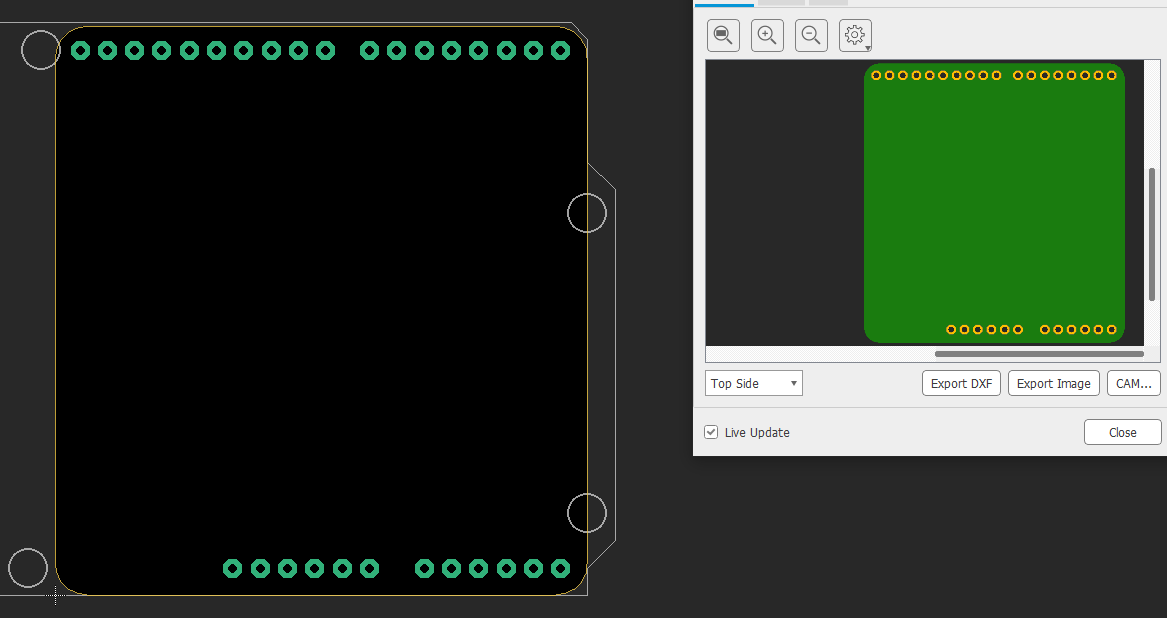
\includegraphics[width=0.7\textwidth, keepaspectratio]{images/shaped.png}
	\caption{This would be a good board shape.}
	\label{fig:shaped}
\end{figure}

\subsection{Positioning the Components}
\subsubsection{Adjusting the grid}
Adjust the grid to 1 mm Size, 0.1 mm Alt just as you did on the lab of Week 2 while creating a footprint. To remind you: You can click on the grid button on the top left and set Size to 1 mm and Alt to 0.1 mm.
\pagebreak
\subsubsection{Drag components}
In this case, you have a lot of space for positioning your components and there's no specific component that has strict positioning constraints try just making the least amount of crossings between airwires. For that, select the moving tool on the left and click on the components to drag them to their positions. You can rotate by pressing the right button.

\begin{figure}[ht]
	\center
	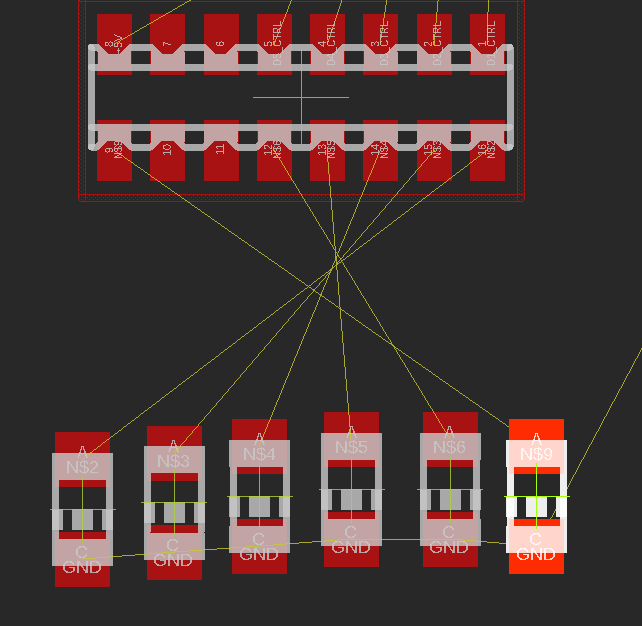
\includegraphics[width=0.4\textwidth, keepaspectratio]{images/cross.png}
	\caption{BAD - Many crossings.}
	\label{fig:cross}
\end{figure}

\begin{figure}[ht]
	\center
	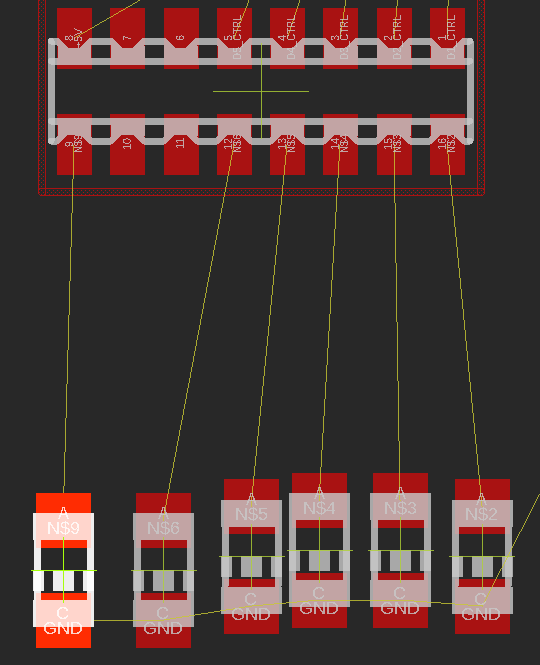
\includegraphics[width=0.4\textwidth, keepaspectratio]{images/no-cross.png}
	\caption{GOOD - No crossings.}
	\label{fig:no-cross}
\end{figure}
\pagebreak
\subsection{Ground Plane}
A polygon plane is important for minimizing the number of traces used for ground and for giving an easy return path for the current current that comes our from your circuitry.
Doing it is quite simple:
\begin{itemize}
\item Make a polygon that covers all of the bottom layer using the Polygon tool on the left. You can do that by making the polygon the same size as the board dimension.
\end{itemize}
\begin{figure}[ht]
	\center
	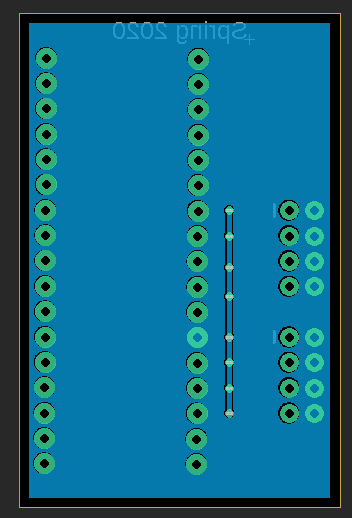
\includegraphics[width=0.4\textwidth, keepaspectratio]{images/groundplane.png}
	\caption{A ground plane example.}
	\label{fig:groundplane}
\end{figure}
\pagebreak
\subsection{Routing}
Use the "Route Airwire" tool to connect all of the airwires. If you need to cross any two traces, you can route a trace underneath the other by putting a via, going to the bottom plane and then, putting another via for the trace to return to the top layer.


\begin{figure}[ht]
	\center
	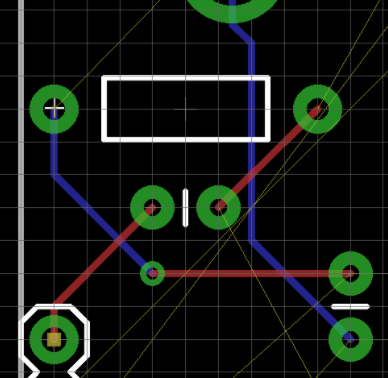
\includegraphics[width=0.4\textwidth, keepaspectratio]{images/undertrace.png}
	\caption{You can route the same signal on different layers.}
	\label{fig:undertrace}
\end{figure}
\subsection{Silkscreen}
Add text on the tPlace layer with the Text tool and, with that, label the LEDs as well as the buttons and the 5V on the 8-pin connector.  
\begin{figure}[ht]
	\center
	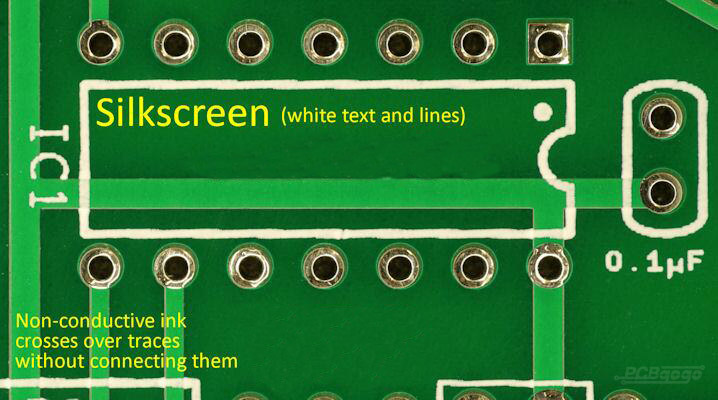
\includegraphics[width=0.4\textwidth, keepaspectratio]{images/silk.png}
	\caption{Silkscreen on a PCB.}
	\label{fig:silkscreen}
\end{figure}
\pagebreak
\subsubsection{Check the Manufacturing Tab}
After that, check on the Manufacturing tab if everything looks good. So, see if there's no silkscreen names or labels under components and see if everything seems informative enough.
\begin{figure}[ht]
	\center
	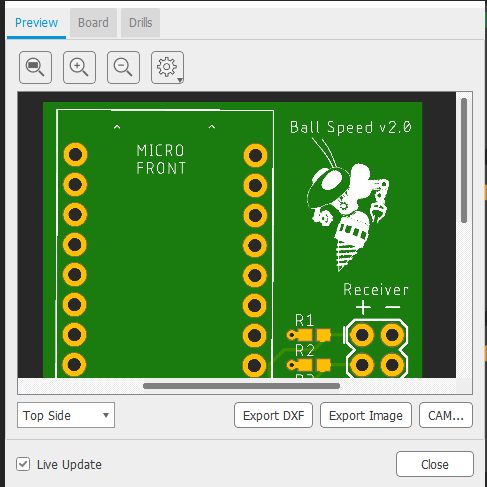
\includegraphics[width=0.4\textwidth, keepaspectratio]{images/manufac.png}
	\caption{This tab should show up after you click on "MANUFACTURING" on the right.}
	\label{fig:manufac}
\end{figure}

\section{Troubleshooting}
To make sure that your board layout design abides by the Design Rules that you have established in the begging of this guide, press the DRC tool on the left and see if a screen appears describing the infractions you have committed. Thus, you can press on the errors and warnings and the screen will take you to them. Make sure you solve every complaint until you are able to press the DRC tool and don't see any warnings/errors.


\section{Resources}
\begin{itemize}
    \item \href{https://www.youtube.com/watch?v=3TP1JzrRRHs&list=PL1R5gSylLha2iQ7e9mwiXJDY2RXoM8HxK&index=4}{EAGLE Board Layout I Video}
    \item \href{https://www.youtube.com/watch?v=w4isa5e_Vow&list=PL1R5gSylLha2iQ7e9mwiXJDY2RXoM8HxK&index=5}{EAGLE Board Layout II Video}
    \item \href{https://github.com/RoboJackets/electrical-training/tree/master/references/eagle_training_guide}{EAGLE Training Guide}
    \item \href{https://wiki.robojackets.org/EAGLE_Style_Guide}{EAGLE Style Guide}
    \item \href{https://github.com/RoboJackets/robocup-firmware/blob/master/doc/Git.md}{Git Guide}
    \item \href{https://github.com/RoboJackets/electrical-training/blob/master/references/eagle_cheat_sheet/eagle_cheat_sheet.pdf}{EAGLE Cheat Sheet}
\end{itemize}


\end{document}